\chapter{SETUP}
\phantomsection
\section{Unpacking and connecting the MEGA65}

Time to set up your MEGA65 home computer.
The box contains the following:
\begin{itemize}
\setlength\itemsep{-0.75mm}
\item MEGA65 computer.
\item Power supply (black box with socket for mains supply).
\item This book, the MEGA65 User's Guide.
\end{itemize}

In addition, to be able to use your MEGA65 computer:
\begin{itemize}
\item A television or computer monitor with a VGA or digital video input, that is capable of displaying an image with 800x600 pixel resolution at 50Hz or 60Hz.
\item A VGA video cable, or;
\item A digital video cable.
\end{itemize}

These items are not included with the MEGA65.

You may also want to use the following to get the most out of your MEGA65:
\begin{itemize}
\item 3.5mm mini-jack audio cable and suitable speakers or hifi system, so that you can enjoy the sound capabilities of your MEGA65.
\item RJ45 Ethernet cable (regular network cable) and a network router or switch. This allows use of the high-speed networking capabilities of your MEGA65.
\end{itemize}

\section{Rear Connections}

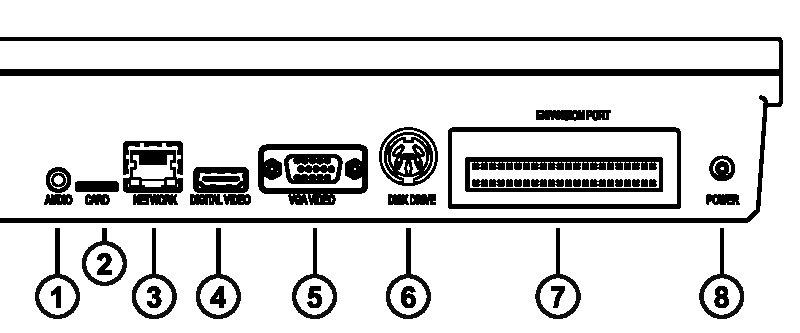
\includegraphics[width=\linewidth]{images/illustrations/mega65-rear.pdf}

\begin{center}
\setlength{\def\arraystretch{1.5}\tabcolsep}{6pt}
\begin{longtable}{ c | l}

	1	& 	3.5mm Audio Mini-Jack \\
	2	& 	SDCard \\
	3	& 	Network LAN Port \\
	4	& 	Digital Video Connector \\
	5	& 	VGA Video Connector \\
	6	& 	External Floppy Disk Drive	\\
	7	& 	Cartridge Expansion Port \\
	8	& 	DC Power-In Socket	 \\

\end{longtable}
\end{center}

\newpage

\section{Side Connections}

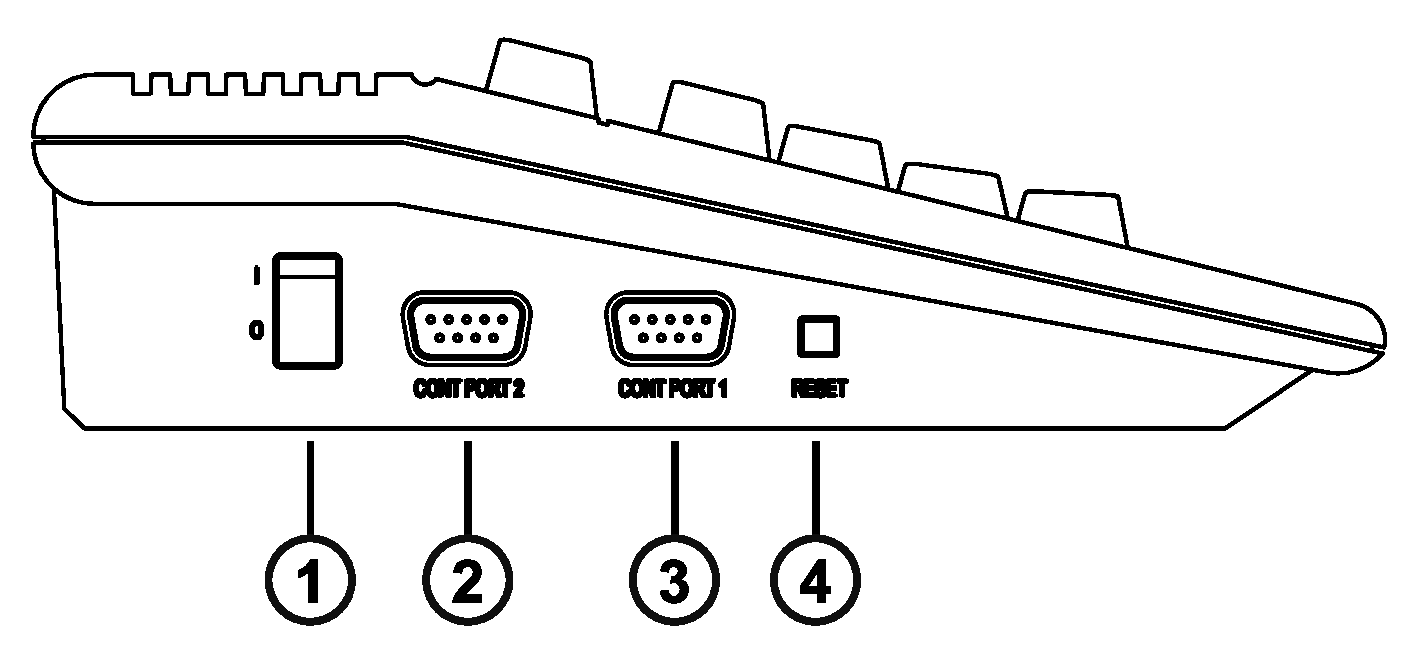
\includegraphics[width=\linewidth]{images/illustrations/mega65-side.pdf}

\begin{center}
\setlength{\def\arraystretch{1.5}\tabcolsep}{6pt}
\begin{longtable}{ c | l}

	1	& 	Power Switch \\
	2	& 	Controller Port 2 \\
	3	& 	Controller Port 1 \\
	4	& 	Reset Button \\

\end{longtable}
\end{center}

Various peripherals can be connected to Controller Ports 1 and 2 such as joysticks or paddles.

\newpage

\section{Installation}

\subsection{Connecting your MEGA65 to a screen and peripherals}

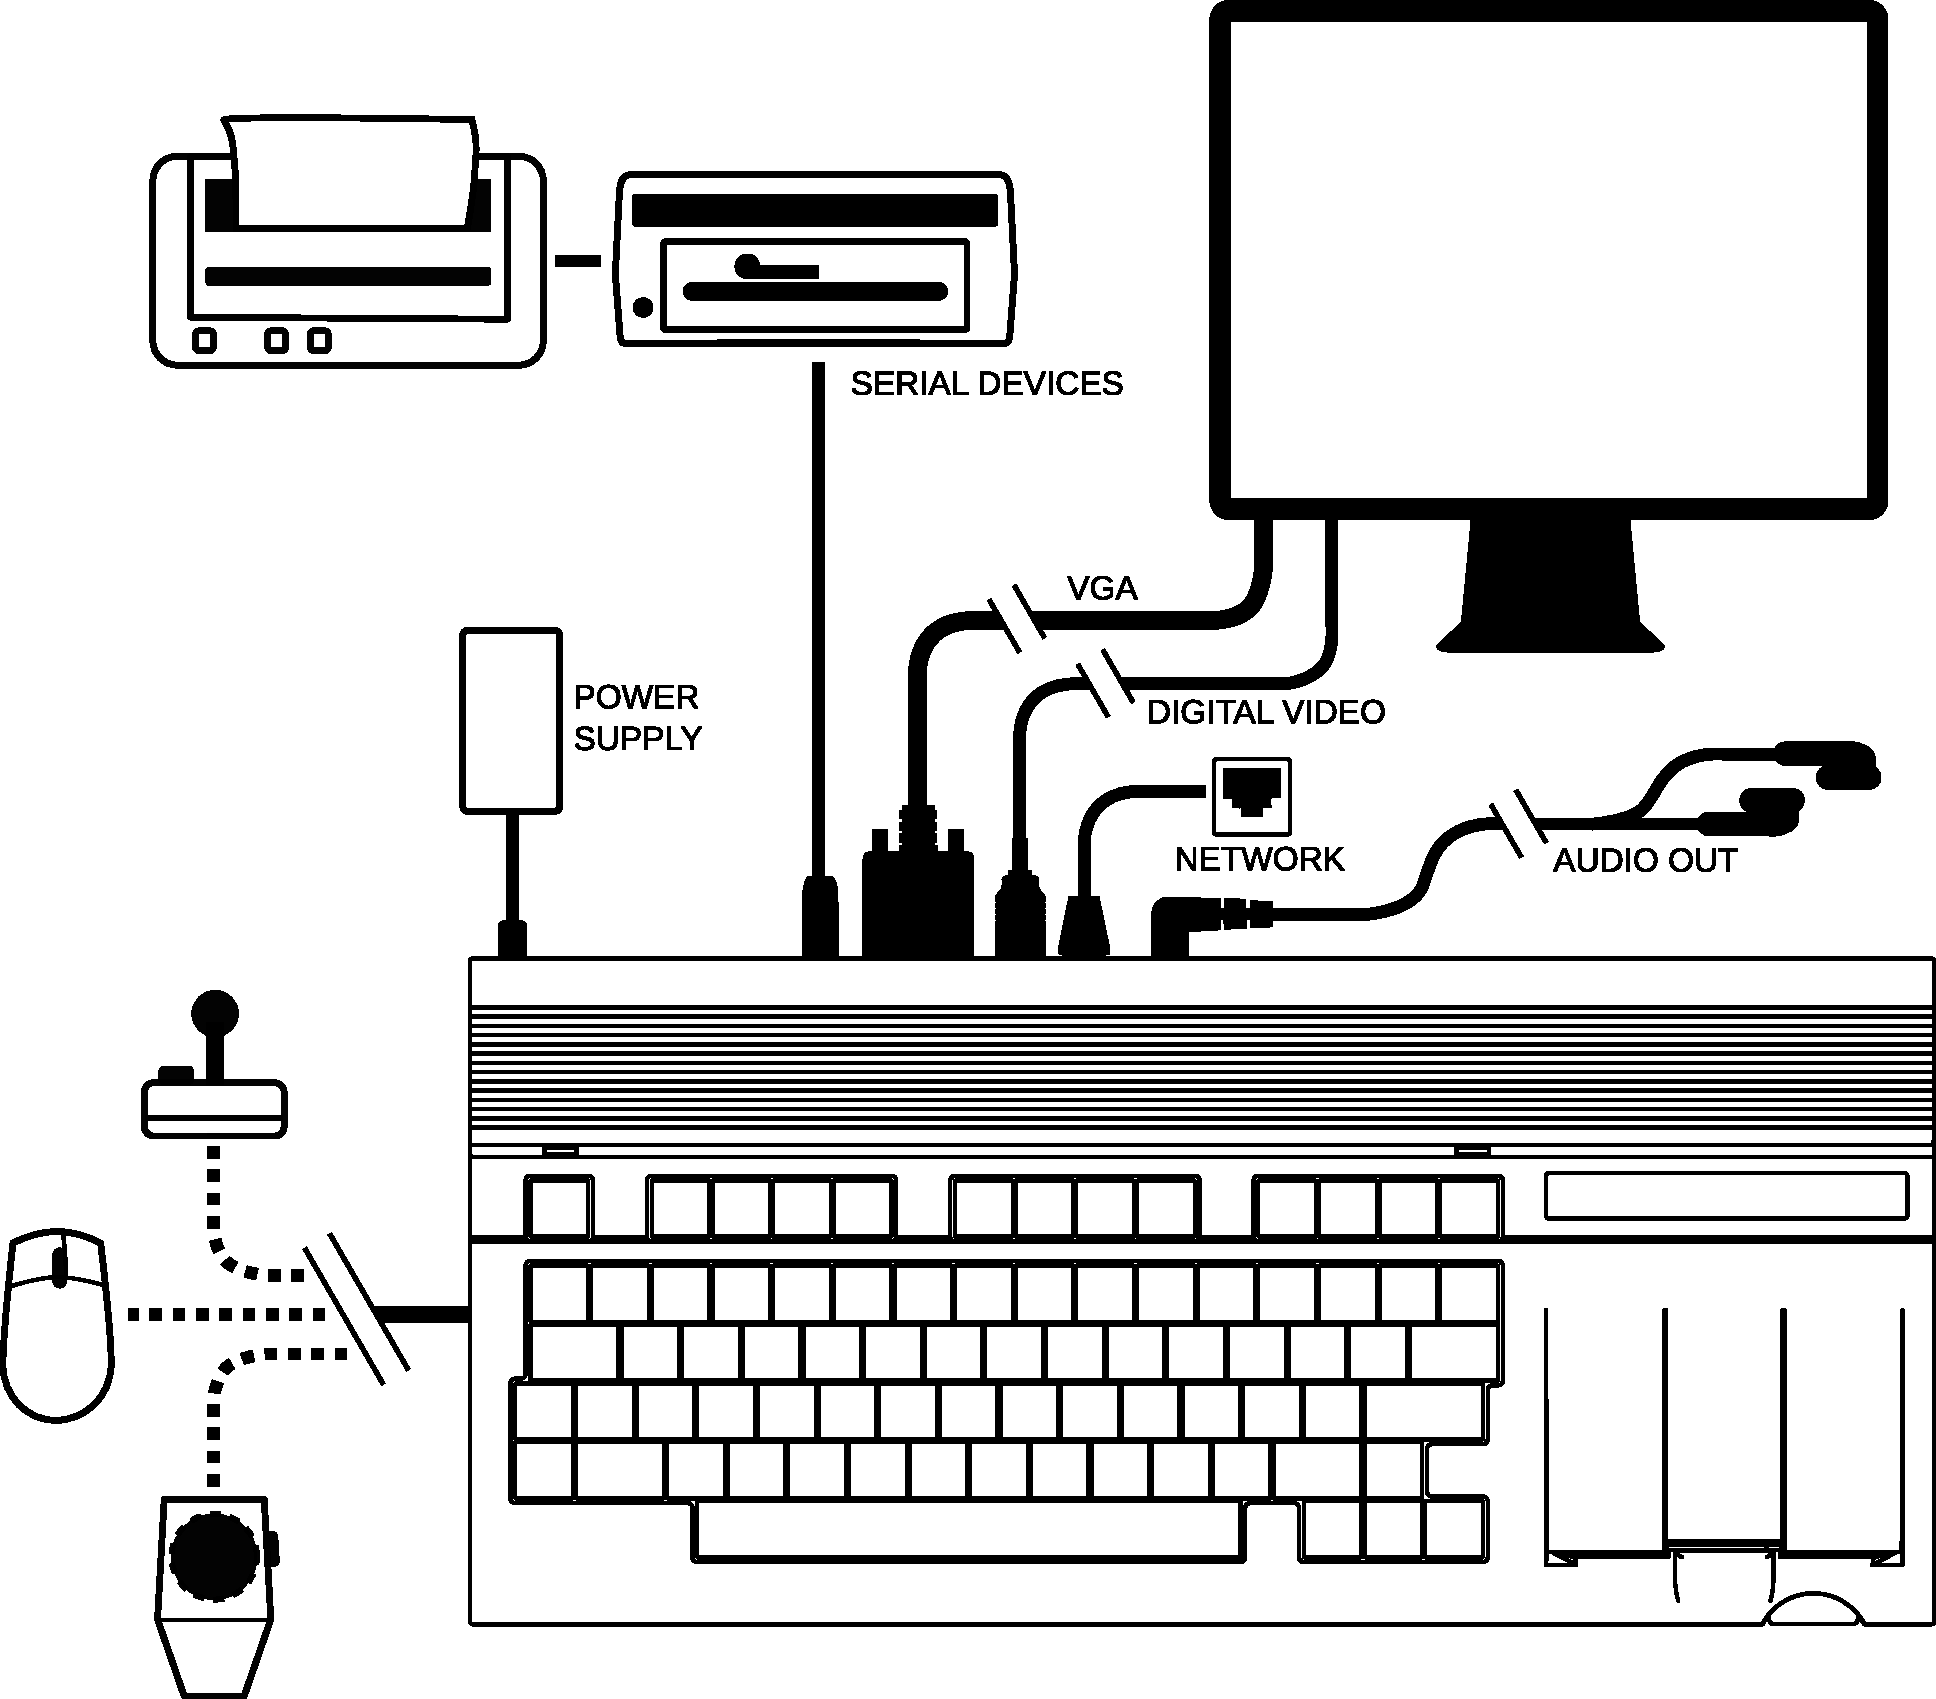
\includegraphics[width=\linewidth]{images/illustrations/mega65-top.pdf}

\newpage

\begin{enumerate}
	\item Connect the power supply to the Power Supply socket of the MEGA65.
	\item If you have a VGA monitor and a VGA cable, connect one end to the VGA port of the MEGA65 and the other end into your VGA monitor.
	\item If you have a TV or monitor with a compatible Digital Video connector, connect one end of your cable to the Digital Video port of the MEGA65, and the other into the Digital Video port of your monitor. If you own a monitor with a DVI socket, you can purchase a DVI to Digital Video adaptor.
\end{enumerate}

\section{Optional Connections}

\begin{enumerate}
	\item The MEGA65 houses an internal 3.5" floppy disk drive. You can also connect older Commodore{\textregistered} IEC serial floppy drives to the MEGA65: the Commodore{\textregistered} 1541, 1571 or 1581. Connect one end of your IEC cable to the Commodore{\textregistered} floppy disk drive and the other end to the Disk Drive socket of the MEGA65. You can also connect SD2IEC devices and PI1541's. It is possible to daisy-chain additional floppy disk drives or Commodore{\textregistered} compatible printers.
	\item You can connect your MEGA65 to a network using a standard Ethernet cable.
	\item For enjoying audio from your MEGA65, you can connect a 3.5mm stereo mini-jack cable to an audio amplifier or speaker system. If your system has RCA connectors you will need to purchase a 3.5mm mini-jack to twin RCA adaptor cable. The MEGA65 also has a built in amplifier to allow connecting headphones.
	\item A Secure Digital Card or SDCard (SDHC and SDXC) can be inserted into the rear of the MEGA65 as a drive.
\end{enumerate}


\section{Operation}

\subsection{Using the MEGA65}

\begin{enumerate}
	\item Turn on the computer by using the switch on the left hand side of the MEGA65.
	\item After a moment, the following will be displayed on your TV or monitor:
\end{enumerate}

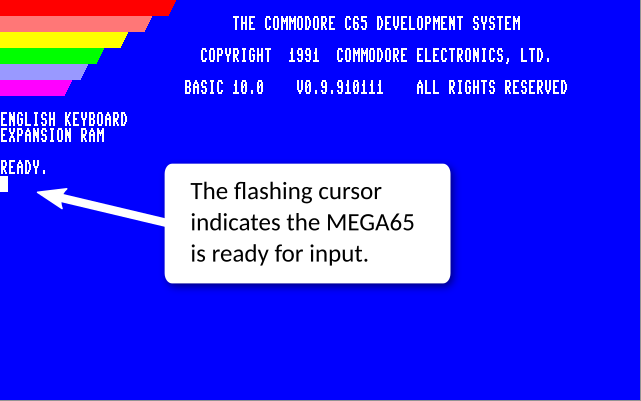
\includegraphics[width=\linewidth]{images/introduction-screen/switched-on.png}

\subsection{THE CURSOR}

The flashing square underneath the READY prompt is called the cursor. The cursor indicates that the computer is ready to accept input. Pressing keys on the keyboard will print that character onto the screen. The character will be printed in the current cursor position, and then the cursor advances to the next position.

You can type commands, for example: telling the computer to load a program. You can even start entering program code.
